\section{Overview}

\TransCal's core comprises of a library of \newterm{rewrite rules} that correlate
equivalent program terms.
A rewrite engine takes a given program term and a \newterm{goal pattern},
and attempts to rewrite the original term such that it matches the pattern,
by exploring the space of consecutive rule applications.
A goal pattern is essentially a term with \newterm{holes} that hold place for
arbitrary subterms, although some semantic constraints are occasionally imposed
on top of it (see later).

While large-scale exhaustive search of all possible rewrites of a program
is highly intractable, it can still be applied locally so that
the user does not have to spell out which rules to apply.
The user usually knows what form they expect the result to be, so specifying
the pattern is natural.

A \newterm{rewrite rule} takes the form $e_1 \dotto e_2$, where $e_1$
and $e_2$ are arbitrary lambda calculus-style terms.
Free variables in $e_1$ are used as wildcards that can be instantiated
to any subexpression, provided that all occurrences of the same variable
are assigned the same term.
If the pattern $e_1$ matches a subterm $s$ of the term subject for rewrite,
that is, $s=\sigma e_1$ for some assignment $\sigma$ to the free variables of $e_1$,
the corresponding instantiation $\sigma e_2$ is inferred to be equivalent to it.
In practice, most rewrite rules are bidirectional, and we use the notation
$e_1 \doteq e_2$ as a shorthand for $e_1 \dotto e_2$, $e_2 \dotto e_1$.

One specific behavior of \TransCal is that terms are never deleted.
Rather than replacing $s$ with $e_2$, both subterms are kept, resulting
in an \newterm{equivalence class}.
These classes are gradually extended as more equivalences are discovered;
the result is a large set of terms, all equivalent to the original program
being refined, compactly represented by a \newterm{Program Equivalence Graph}
structure.

From this space of possible programs, the system would eventually select
one according to some optimality criteria.
This is when \TransCal enters interactive mode: the user specifies such
desired properties via a \newterm{goal predicate}.
\TransCal supports three types of goal predicates:
\begin{itemize}
  \item Elaboration --- a template (program term with holes) for the resulting
    program.
    The holes represent any term, and can be named like in rewrite patterns.
  \item Generalization --- a set of terms that restricts variables appearing
    as leaves of the resulting term. For example, $\langle h\,x, y\rangle$
    means that $x$ is only allowed to occur as part of a subterm $h\,x$,
    whereas $y$ is allowed to occur free regardless of context, and no other
    variables should appear in the term.
    Generalization introduces a new name $f$ such that $f\,(h\,x)\,y \equiv s$
    ($s$ is the subterm being rewritten),
    and a closed definition $f = \alpha\,\beta \mapsto \ldots$.
  \item Rippling --- 
\end{itemize}

\subsection{Example}

As a motivation, we look at Bird's Functional Pearl~\cite{bird2006functional},
where one of the core functions is defined (in Haskell) as

\begin{lstlisting}[mathescape]
nodups :: Eq a $\Rightarrow$ [a] $\to$ Bool
nodups [] = True
nodups (x : xs) = notElem x xs $\land$ nodups xs
\end{lstlisting}

The function \lstinline!notElem! is defined in the Haskell standard library as:

\begin{lstlisting}[mathescape]
notElem x = not . elem x
\end{lstlisting}

The program in question was written to be short and elegant, but also
efficient. Still, the function \lstinline!nodups! was somewhat overlooked,
and an acute reader can easily discern that it runs in quardatic time
(in the length of the list). For the application in question (a Sudoku solver),
the lists are of length 9 or less; but for general use, a more efficient
version would be desirable. Moreover, we would like to do this without
compromising the succinctness of Bird's formulation. For this purpose,
assume \lstinline!nodups! above is the \emph{specification}, and we show how
a user would effectively derive implementation by rewrite.

The core insight of this derivation is that iterated elements can be stored
in a hash, a set data structure that offers fast lookup.
It would allow to compute \lstinline!notElem! in constant time.
However, the way the specification above is written, it is hard to figure out
how to use the hash, because the set of elements being tested (\lstinline!xs!)
is different in each invocation.
A rephrasing is needed to expose useful structure.

We lay out the steps informally, and then show two ways in which \TransCal
tactics can be used to formalize it.

\newcommand\xs{\symvar{xs}}
\newcommand\nodups{\symfun{nodups}}
\newcommand\notElem{\symfun{notElem}}
\newcommand\elem{\symfun{elem}}
\newcommand\ys{\symvar{ys}}

\begin{itemize}
\item
The test \lstinline!notElem x xs!
can be phrased as $x \not\in \widehat{\xs}$, where $\widehat{\xs}$ denotes
the set of elements in $xs$.
This is equivalent to $\{x\} \parallel \widehat{\xs}$, where $\parallel$
denotes set disjointness.
\item
Generalize the resulting right-hand side as $\nodups' \, \{x\} \; \xs$,
  where $\nodups' = a\,\xs \mapsto a\parallel\widehat{\xs} \land \nodups\;\xs$.
\item 
If $xs=[]$, both conjuncts are trivially false.
Assume therefore $\xs = x' : \xs'$ for some $x'$ and $\xs'$ of the appropriate
types.
\item
$a \parallel \widehat{x':\xs'}$ can be unfolded to
$x'\not\in a \land a \parallel \widehat{\xs'}$.
\item $\nodups~(x':\xs')$ can be unfolded to
$\notElem~x'~\xs' \land \nodups~\xs'$. The last two unfolds give:
\[x'\not\in a \land a \parallel \widehat{\xs'} \land
  \notElem~x'~\xs' \land \nodups~\xs'\]
\item Use associativity and rewrite the two middle conjuncts:
\[a \parallel \widehat{\xs'} \land
  \notElem~x'~\xs' 
  \;\;\;{\equiv}\;\;\;
  a \parallel \widehat{\xs'} \land
  \{x'\} \parallel \widehat{\xs'}
  \;\;\;{\equiv}\;\;\;
  \big(a \cup \{x'\}\big) \parallel \widehat{xs'}\]
The expression becomes
\[x'\not\in a ~\land~ \big(a \cup \{x'\}\big) \parallel \widehat{xs'}
  ~\land~ \nodups~\xs'\]
\item Notice that the last two conjuncts constitute $\nodups'\,(a\cup\{x'\})\;\xs'$.
  Conclude
\[\nodups'\,a\;(x'\!{:}\xs') \;\;=\;\; x'\not\in a ~\land~ \nodups'\,(a\cup\{x'\})\;\xs'\]
which gives a recursive implementation of $\nodups'$.
\end{itemize}

\bigskip
Evidently, expressing the refinement steps in English is rather cumbersome.
Since the transformations are algebraic in nature, a more mathematical
language would be better.
As an appetizer, we display the same development in annotated form in
\Cref{nodups:proof-sketch-1}.
Braces are used to mark up subterms being rewritten.

\begin{figure}[b]
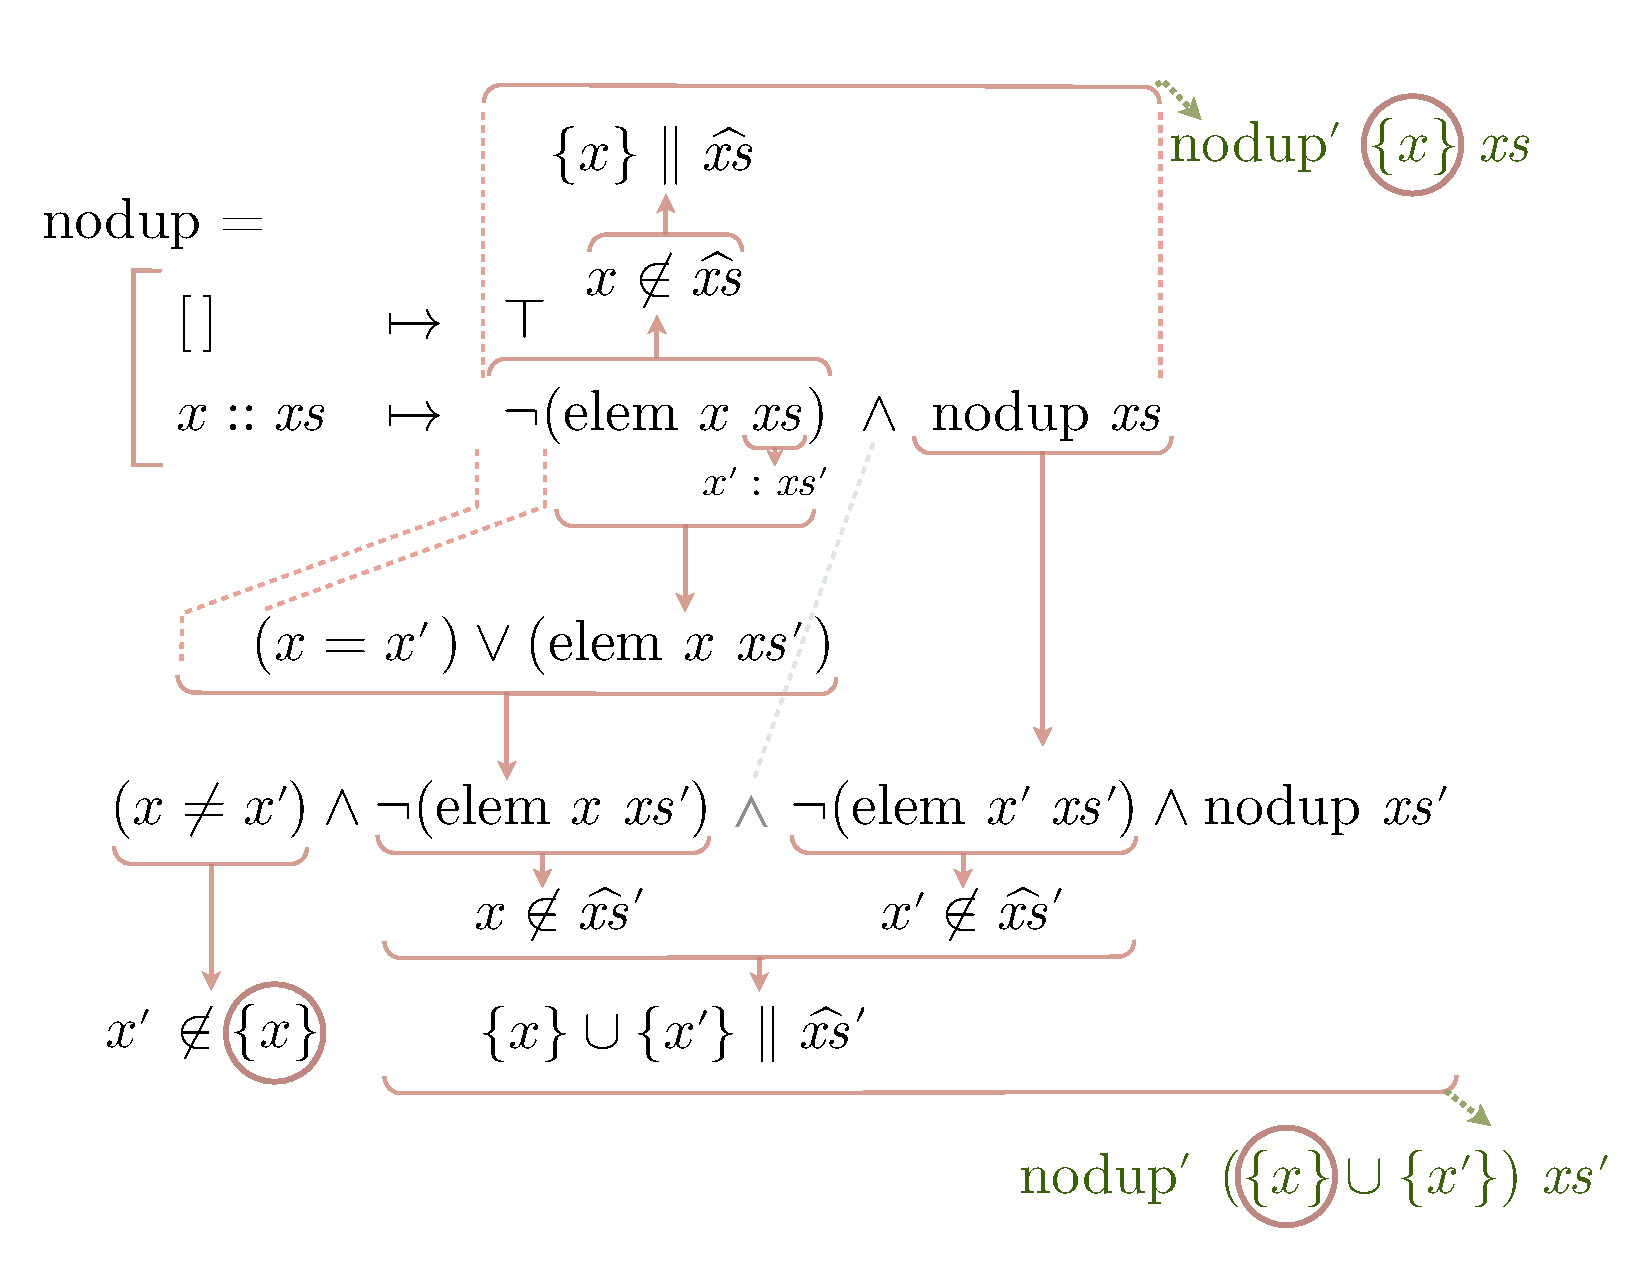
\includegraphics[width=0.6\textwidth]{gfx/nodup-1-placeholder}
\caption{\label{nodups:proof-sketch-1} Development}
\end{figure}

\begin{table}
\[\begin{array}{rcl}
    \elem~x~\lnil       & \dotto &  \bot                   \\
    \elem~x~(y:\ys)     & \doteq &  x=y \lor \elem~x~\ys   \\
    \elem~x~\ys         & \doteq &  x \in \widehat{\ys}    \\
    \notElem~x~\ys      & \doteq &  \lnot \elem~x~\ys      \\
    x\neq y             & \doteq &  \lnot(x = y)           \\
    x\not\in y          & \doteq &  \lnot(x \in y)         \\
    x \in \{y\}         & \doteq &  x = y                  \\
    x \parallel \{y\}   & \doteq &  y \not\in x            \\
    x \land (y\land z)  & \doteq &  x\land y\land z        \\
    \lnot(x\land y)     & \doteq &  \lnot x \lor \lnot y   \\
    \lnot(x\lor y)      & \doteq &  \lnot x \land \lnot y  \\
    x\parallel y \land
    x\parallel z        & \doteq &  x \parallel (y\cup z)  \\
    x\parallel z \land
    y\parallel z        & \doteq &  (x\cup y) \parallel z  \\
  \end{array}\]
\caption{\label{basic-rules}}
\end{table}
